\documentclass[aps,reprint,prl]{revtex4-1}
\usepackage{graphicx}  % needed for figures
\usepackage{dcolumn}   % needed for some tables
\usepackage{bm}        % for math
\usepackage{amssymb,amstext,amsmath}   % for math
\usepackage{url}
\usepackage{hyperref}

\begin{document}
\title{Dark Matter Particle Detection: A Review}
\author{Steven Kaplan}
\affiliation{Department of Physics and Astronomy, Rutgers, The State University of New Jersey, 136 Frelinghuysen Road, Piscataway, New Jersey 08854, USA}

\begin{abstract}
Dark matter detection efforts in the particle physics realm are vast and comprise many different methods.  From galactic rotation curves and limits on $\Omega_m$ from Big Bang Nucleosynthesis and Cosmic Microwave Background measurements, there is very strong evidence for the existence of dark matter.  This paper will focus on the hypothesis that dark matter is made of Weakly Interacting Massive Particles (WIMPs).  Light supersymmetric particles such as the neutralino are seen as a natural choice for a dark matter candidate. There are many experiments devoted to discovering dark matter either directly though an interaction between the hypothetical WIMP and the nucleus of an atom in the detector or indirectly through the discovery of an excess of the WIMPs possible decay products.  Following this is a treatment of the detection methods themselves.  The results of these experiments have proven to be controversial, as any purported discovery is located in the exclusion zone of the Large Underground Xenon experiment (LUX) among others.
\end{abstract}

\maketitle
\subsection*{Introduction And Motivation}
For the past many decades, a great amount research has been done in cosmology to answer seemingly simple questions: can we confirm that dark matter exists and, if it does, what are its properties?  There is a great deal of evidence that dark matter does, indeed, exist.  Considering the luminous matter in galaxies, the mass is mostly concentrated in the center, and the density falls as one looks further away from the center.  Very naively, I distill the dynamics of the galaxy to two point masses $m$ and $M$ with $m\ll M$ where the mass $m$ has a circular orbit with velocity $v$ around the mass $M$.  In this case, we know that 
$$\frac{GmM}{r^2}=\frac{mv^2}{r}\;.$$
This implies that $v\propto r^{-1/2}$.  An assumption that the galaxy is in viral equilibrium leads to the same conclusion \cite{TASIOlive}.
\begin{figure}[h]
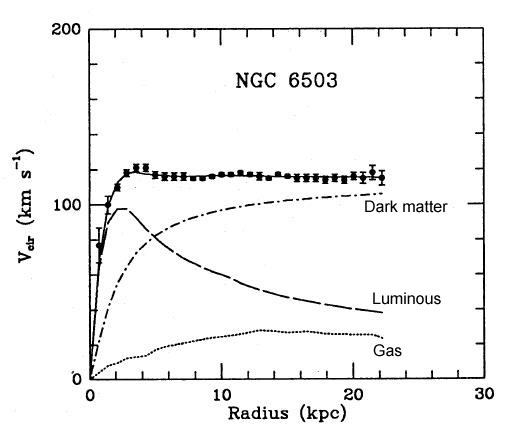
\includegraphics[width=0.5\textwidth]{rotationcurve}
\caption{Rotation curve of NGC 6503 taken from \cite{begman}.  This clearly shows that the data does not fit the null hypothesis of the galaxy consisting of only luminous matter.}
\label{fig:rotationcurve}
\end{figure}
Measurements of galactic rotation curves show results that are inconsistent with this assessment. Without questioning our understanding of gravity at galactic scales, this problem can be solved by positing that there is a non-luminous halo of matter surrounding the galaxy in question.  This would give rise to a nearly flat rotation curve as is shown in figure \ref{fig:rotationcurve} to fit the data very well.
\\ \\
Another piece of evidence for the existence of dark matter comes from Big Bang Nucleosynthesis (BBN) and observations of the Cosmic Microwave Background (CMB).  $\Omega_m$ is constrained to be around 0.3, yet baryonic matter only accounts for about 1/6 of this.  Clearly there must be non-baryonic matter that does not couple to electromagnetism (hence dark matter). 
\subsection*{Detection Methods}

The detection of particle dark matter can be divided mainly into two categories: direct and indirect detection.  Direct detection involves the scattering of the dark matter candidate against the nucleus of an atom in the detector.  Under the assumption that the DM halo of the Milky Way is comprised of WIMPs, then the incident flux of WIMPs on Earth is on the order of $10^5$ cm$^{-2}$s$^{-1}$ assuming a WIMP mass of 100 GeV \cite{BertoneBook}.  This seems quite high until the WIMP-nucleon cross section is considered.  A ballpark assumption of the WIMP-nucleon cross section to be on the order of $10^{-37}$ cm$^2$ brings the expected event yield quite low.  The expected event yield ranges from $10^{-5}$ to about 10 events per kg of detector per day.  As such, extreme care must be taken to understand and eliminate background events.  To actualize this, direct detection experiments are mainly situated deep underground in order to drastically cut the cosmic ray background, and the detector material is kept cold to quell the effect of thermal excitation of the detector material \cite{encyclo}.
%\\ \\
%Indirect detection involves the detection of either the annihilation or decay products of the dark matter candidate.
\subsection*{Detector Setups}
This section will briefly discuss the experimental setup of various dark matter detection experiments.  I start with the direct detection experiments: CDMS, CoGeNT, XENON, LUX, et. al.  The CDMS experiment (and other semiconductor experiments such as CoGeNT) operate at near absolute zero temperatures ($\sim 40$ mK in the case of CDMS \cite{queens}).  When a WIMP enters the detector, there is a thermal excitation in the material that is a function of the WIMP energy.  CDMS can also measure the level of ionization caused by an incoming particle.  The level of thermal excitation relative to the level of ionization for a given event provides a way to distinguish between the WIMP signal and the background \cite{wiki:cdms}.  XENON and LUX are Time Projection Chambers (TPCs).  The detector material in both cases is liquid Xenon with a layer of gaseous Xenon above.  When a particle enters the detector material, scintillation photons are released and detected by photomultiplier tubes (referred to as the S1 signal).  Electrons are also ionized and are forced by an electric field to travel through the gaseous Xenon.  These electrons also have a scintillation signal (referred to as S2).  S2/S1 can be used as a discriminating variable between a nuclear recoil from the WIMP signal and ionization from radiation \cite{BertoneBook,wiki:xenon}.  

\subsection*{Results}
\begin{figure}[h]
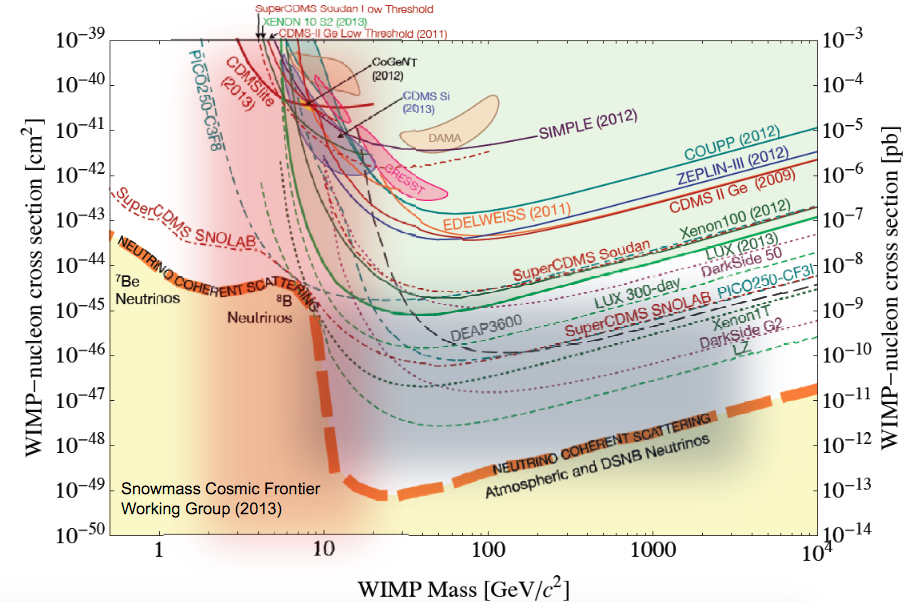
\includegraphics[width=0.5\textwidth]{dmsearchresults}
\caption{This plot, taken from a talk by \cite{feng}, summarizes the results of many dark matter searches.  The open lines are upper limits on the WIMP-nucleon cross section while closed curves denote possible dark WIMP detections.}
\label{fig:res}
\end{figure}
Figure \ref{fig:res} summarizes the results of many dark matter searches.  It should be noted that the searches represented here are not comparable in the strictest sense.  For example, CDMS and CoGeNT are comprised of a germanium (silicon as well in the case of CDMS) detector while experiments like XENON and LUX use liquid and gaseous Xenon.  What is clear here is that there is a contradiction in the results.  All of the experiments who claim a detection (CDMS, DAMA, CoGeNT, CRESST) are located in the excluded zones of at least one other experiment.  The 2013 LUX result appears to exclude all of the detections.
\begin{figure}[h]
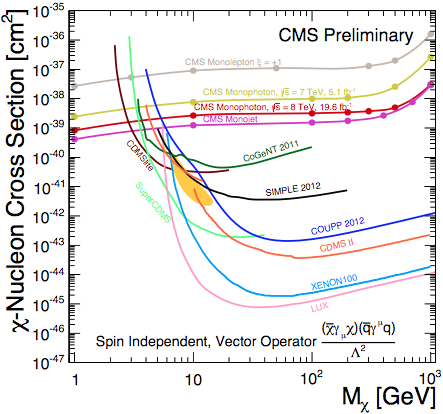
\includegraphics[width=0.5\textwidth]{cmsdmresults}
\caption{This plot is taken from \cite{zeynep}.  Shown is the upper limit on the spin independent WIMP-nucleon cross sections from various experiments.  Some are the same curves as shown in figure \ref{fig:res}.  What should be noted here is that collider experiments such as CMS are currently able to probe lower in WIMP mass than direct detection experiments.}
\label{fig:cmsres}
\end{figure}
\\ \\
Shown in figure \ref{fig:cmsres} are the results from dark matter searches from the Compact Muon Solenoid (CMS) experiment a the Large Hadron Collider (LHC).  While direct dark matter searches are able to exclude lower WIMP-nucleon cross sections, CMS has the advantage of being able to exclude cross sections for a larger range of WIMP mass.
\newpage
\bibliographystyle{unsrt}
\bibliography{finalSources}
\end{document}